\newpage
\section{Introdução}
\label{sec:introducao}

\textcolor{violet}{Nesta seção você deve falar em  qual contexto seu trabalho está inserido. 
Qual o problema que está sendo abordado e qual a proposta de solução (em linhas gerais). 
Qual a motivação/justificativa para o desenvolvimento da solução proposta (Dentre as possibilidades de solução porque essa foi a escolhida). O texto pode ser dividido em subseções.} 
\subsection{Contexto}
\subsection{Problema e solução proposta}
\subsection{Justificativa}

Exemplo de referência para figura

Como visto na Figura~\ref{fig:lifecycle_phase} $\ldots$

\begin{figure}[ht]
    \center
    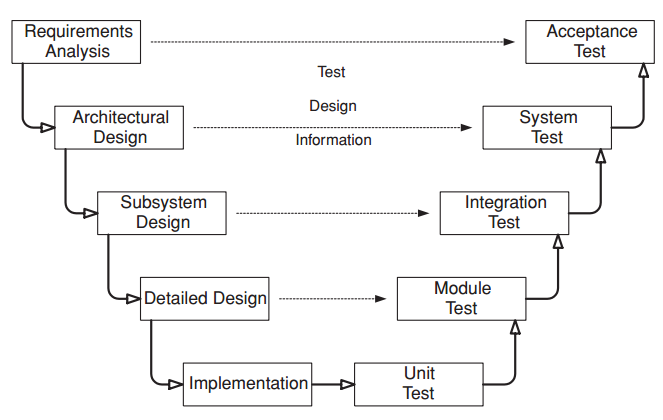
\includegraphics[scale=0.7]{images/lifecycle_phase.png}
    \caption{Testing levels based on software development phase (Sommerville, 2011).}
    \label{fig:lifecycle_phase}
\end{figure}

Exemplo de referência para bibliografia

De acordo com \cite{sommerville2011software} $\ldots$

Exemplo de citação bibliográfica.\cite{WCAG}
